% F091｜完全立方数的立方根尾数速判｜02_explanation.tex
% 继承上传模板的 LaTeX 环境；当前条目的内容独立编写。
\clearpage
\begin{explanationbox}
\textbf{\textcolor{CExplanation}{为什么个位不会受十位影响}}
\par\medskip
\begin{center}
% F091｜last 原创简明教学示意图
\begin{tikzpicture}[>=stealth,scale=.89]
\node[draw,rounded corners,fill=teal!9,minimum width=3cm] (a) at (0,0){$7^3=343$};
\node[draw,rounded corners,fill=orange!9,minimum width=3cm] (b) at (4.1,0){尾数 $3$};
\node[draw,rounded corners,fill=teal!15,minimum width=3cm] (c) at (8.2,0){根的个位 $7$};
\draw[->,thick] (a)--(b);\draw[->,thick] (b)--(c);
\end{tikzpicture}

\end{center}
\medskip
把两位整数写成 $10m+u$。由立方公式，$(10m+u)^3=1000m^3+300m^2u+30mu^2+u^3$；前面三项都有因数 $10$，因此个位只取决于 $u^3$ 的个位。
\end{explanationbox}
\clearpage
\begin{explanationbox}
\textbf{\textcolor{CExplanation}{为什么左侧的103能定十位}}
\par\medskip
\begin{center}
% F091｜split 原创简明教学示意图
\begin{tikzpicture}[>=stealth,scale=.9]
\node[draw,rounded corners,fill=teal!9,minimum width=2.5cm,minimum height=1.25cm] (a) at (0,0){$\underbrace{103}_{\text{高位}}\mid\underbrace{823}_{\text{低位}}$};
\node[draw,rounded corners,fill=orange!9,minimum width=3.2cm,minimum height=1.25cm] (b) at (4.5,0){$4^3\le103<5^3$};
\node[draw,rounded corners,fill=teal!15,minimum width=2.3cm,minimum height=1.25cm] (c) at (9.0,0){$\sqrt[3]{103823}=47$};
\draw[->,thick] (a)--(b);\draw[->,thick] (b)--(c);
\node at (4.5,-1.2){\small 高位定十位，末位定个位};
\end{tikzpicture}

\end{center}
\medskip
若根是 $10m+u$ 且 $0\le u\le9$，就有 $(10m)^3\le N<[10(m+1)]^3$。两边除以1000，得 $m^3\le N/1000<(m+1)^3$。因此左侧整数 $H=\lfloor N/1000\rfloor$ 满足 $m^3\le H<(m+1)^3$。
\end{explanationbox}
\clearpage
\begin{explanationbox}
\textbf{\textcolor{CExplanation}{为什么必须是完全立方}}
\par\medskip
\begin{center}
% F091｜verify 原创简明教学示意图
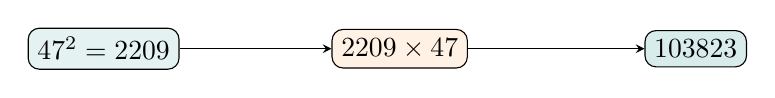
\begin{tikzpicture}[>=stealth,scale=.94]
\node[draw,fill=teal!10,rounded corners] (a) at (0,0){$47^2=2209$};
\node[draw,fill=orange!10,rounded corners] (b) at (4,0){$2209\times47$};
\node[draw,fill=teal!15,rounded corners] (c) at (8,0){$103823$};
\draw[->] (a)--(b);\draw[->] (b)--(c);
\end{tikzpicture}

\end{center}
\medskip
$103823$ 可由数位规则得到候选 $47$，再验 $47^3=103823$。如果 $N$ 不是完全立方，左侧和个位规则仍可能给出一个“候选整数”，但不能当作精确的立方根。
\end{explanationbox}
